\documentclass[
11pt, % The default document font size, options: 10pt, 11pt, 12pt
codirector, % Uncomment to add a codirector to the title page
]{charter} 


% El títulos de la memoria, se usa en la carátula y se puede usar el cualquier lugar del documento con el comando \ttitle
\titulo{Monitoreo y control de sistemas de bombeo de agua potable de pozos profundos} 

% Nombre del posgrado, se usa en la carátula y se puede usar el cualquier lugar del documento con el comando \degreename
\posgrado{Maestría en Sistemas Embebidos} 
%\posgrado{Carrera de Especialización en Internet de las Cosas} 
%\posgrado{Carrera de Especialización en Inteligencia Artificial}
%\posgrado{Maestría en Sistemas Embebidos} 
%\posgrado{Maestría en Internet de las cosas}
% IMPORTANTE: no omitir titulaciones ni tildación en los nombres, también se recomienda escribir los nombres completos (tal cual los tienen en su documento)
% Tu nombre, se puede usar el cualquier lugar del documento con el comando \authorname
\autor{Esp. Ing. Mario Fernando Aguilar Montoya}

% El nombre del director y co-director, se puede usar el cualquier lugar del documento con el comando \supname y \cosupname y \pertesupname y \pertecosupname
\director{Mg. Ing. Mauricio Barroso Benavides}
\pertenenciaDirector{FIUBA} 
%\codirector{Título y Nombre del codirector} % para que aparezca en la portada se debe descomentar la opción codirector en los parámetros de documentclass
%\pertenenciaCoDirector{FIUBA}

% Nombre del cliente, quien va a aprobar los resultados del proyecto, se puede usar con el comando \clientename y \empclientename
\cliente{Ing. Carlos Alvarado Cruz}
\empresaCliente{COSAALT RL}
 
\fechaINICIO{22 de junio de 2024}		%Fecha de inicio de la cursada de GdP \fechaInicioName
\fechaFINALPlan{17 de Agosto de 2024} 	%Fecha de final de cursada de GdP
\fechaFINALTrabajo{15 de mayo de 2025}	%Fecha de defensa pública del trabajo final


\begin{document}

\maketitle
\thispagestyle{empty}
\pagebreak


\thispagestyle{empty}
{\setlength{\parskip}{0pt}
\tableofcontents{}
}
\pagebreak


\section*{Registros de cambios}
\label{sec:registro}


\begin{table}[ht]
\label{tab:registro}
\centering
\begin{tabularx}{\linewidth}{@{}|c|X|c|@{}}
\hline
\rowcolor[HTML]{C0C0C0} 
Revisión & \multicolumn{1}{c|}{\cellcolor[HTML]{C0C0C0}Detalles de los cambios realizados} & Fecha      \\ \hline
0      & Creación del documento                                 &\fechaInicioName \\ \hline
1      & Se completa hasta el punto 9 inclusive                & {2} de {agosto} de 2024 \\ \hline
%2      & Se completa hasta el punto 9 inclusive
%		  Se puede agregar algo más \newline
%		  En distintas líneas \newline
%		  Así                                                    & {día} de {mes} de 202X \\ \hline
%3      & Se completa hasta el punto 12 inclusive                & {día} de {mes} de 202X \\ \hline
%4      & Se completa el plan	                                 & {día} de {mes} de 202X \\ \hline

% Si hay más correcciones pasada la versión 4 también se deben especificar acá

\end{tabularx}
\end{table}

\pagebreak



\section*{Acta de constitución del proyecto}
\label{sec:acta}

\begin{flushright}
Buenos Aires, \fechaInicioName
\end{flushright}

\vspace{2cm}

Por medio de la presente se acuerda con el \authorname\hspace{1px} que su Trabajo Final de la \degreename\hspace{1px} se titulará ``\ttitle'' y consistirá en esencialmente en la implementación de un prototipo de un sistema para el monitoreo y control de un sistema de bombeo de agua potable. El trabajo tendrá un presupuesto preliminar estimado de 680 hs de trabajo y un costo estimado de 46358 Bs, con fecha de inicio el \fechaInicioName\hspace{1px} y fecha de presentación pública el \fechaFinalName.

Se adjunta a esta acta la planificación inicial.

\vfill

% Esta parte se construye sola con la información que hayan cargado en el preámbulo del documento y no debe modificarla
\begin{table}[ht]
\centering
\begin{tabular}{ccc}
\begin{tabular}[c]{@{}c@{}}Dr. Ing. Ariel Lutenberg \\ Director posgrado FIUBA\end{tabular} & \hspace{2cm} & \begin{tabular}[c]{@{}c@{}}\clientename \\ \empclientename \end{tabular} \vspace{2.5cm} \\ 
\multicolumn{3}{c}{\begin{tabular}[c]{@{}c@{}} \supname \\ Director del Trabajo Final\end{tabular}} \vspace{2.5cm} \\
\end{tabular}
\end{table}




\section{1. Descripción técnica-conceptual del proyecto a realizar}
\label{sec:descripcion}

En los últimos años la tendencia tecnológica se ha orientado hacia la creación de dispositivos electrónicos conectados a internet. Permitiendo la implementación de una amplia variedad de nuevas aplicaciones.

Cossalt RL es una cooperativa que da el servicio de agua a la ciudad de Tarija. Actualmente la cooperativa consta de 50 sistemas de bombeo de agua de pozos distribuidos por toda la ciudad para poder suministrar agua potable a las personas de cada zona. La mayoría de los sistemas son manuales esto quiere decir que hay un operario que se encarga de prender y apagar las bombas de agua dependiendo el nivel del agua en los tanques de almacenamiento todo de forma manual.

El objetivo principal del proyecto es la creación de un sistema capaz de realizar mediaciones de consumo eléctrico de las bombas, presión del agua en las tuberías, nivel del tanque de almacenamiento y enviar los datos obtenidos a una plataforma IoT haciendo uso de un módulo de comunicación GSM/GPRS. El sistema también controlara el encendido y apagado de las bombas de forma automática dependiendo las lecturas de los sensores. La plataforma IoT permitirá almacenar los datos, crear paneles de visualización y controlar actuadores. También se mostrarán los datos obtenidos en un display ubicado en el panel de control.
En la figura \ref{fig:diagra_sistema} se puede observar el diagrama de bloques del sistema.

El proyecto permitirá al cliente disminuir el desperdicio de agua que ocurre al momento de bombear agua desde los pozos profundos a los tanques de almacenamiento, también ayudará a detectar de forma temprana posibles rupturas en las tuberías. Al tener un monitoreo y control del encendido y apagado de las bombas se disminuira el consumo eléctrica.

\begin{figure}[hpb]
	\centering 
	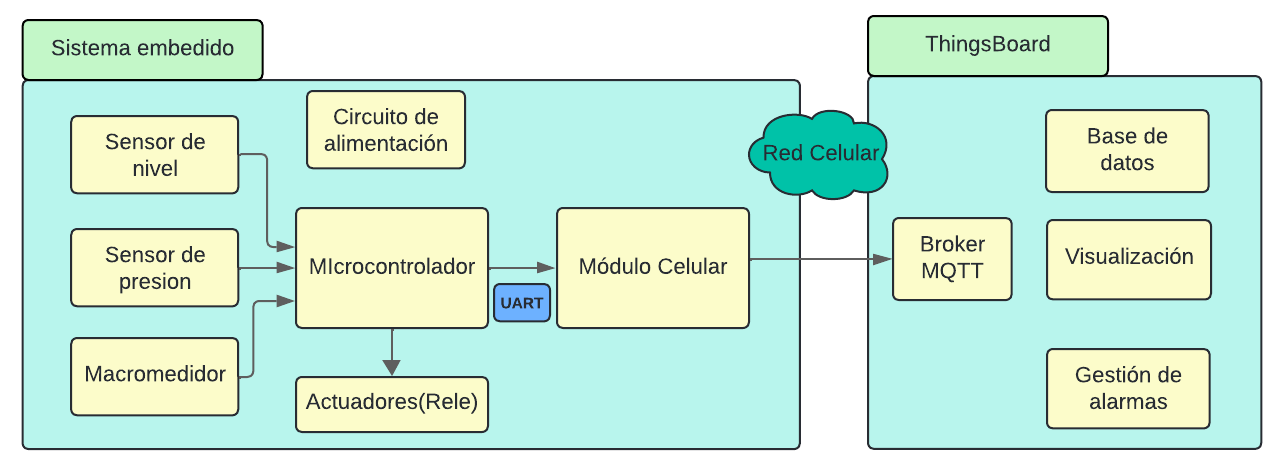
\includegraphics[width=15cm, height=8.5cm]{./Figuras/d_sistema.png}
	\caption{Diagrama en bloques del sistema.}
	\label{fig:diagra_sistema}
\end{figure}
\vspace{2cm}



\section{2. Identificación y análisis de los interesados}
\label{sec:interesados}

\begin{table}[ht]
%\caption{Identificación de los interesados}
%\label{tab:interesados}
\begin{tabularx}{\linewidth}{@{}|l|X|X|l|@{}}
\hline
\rowcolor[HTML]{C0C0C0} 
Rol           & Nombre y Apellido & Organización 	& Puesto 	\\ \hline
Cliente       & \clientename      &\empclientename	& Operador de sistema de bombeo      	\\ \hline
Responsable   & \authorname       & FIUBA        	& Alumno 	\\ \hline
Orientador    & \supname	      & - 				& Director del Trabajo Final \\ \hline
Usuario final & Operarios         & COSAALT RL            	& -      	\\ \hline
\end{tabularx}
\end{table}

\begin{itemize}
	\item Orientador: El Mg. Ing. Mauricio Barroso Benavides tiene mucha experiencia en el desarrollo de proyectos IoT, será una guía para el desarrollo del firmware y del hardware del embebido. Es exigente con los tiempos y la
	calidad del desarrollo del proyecto.
\end{itemize}



\section{3. Propósito del proyecto}
\label{sec:proposito}
El propósito del proyecto es desarrollar un sistema que sea capaz de monitorear y controlar parámetros relevantes en un sistema de bombeo de agua, con la finalidad de disminuir el consumo energético de las bombas  y el desperdicio de agua potable.

\section{4. Alcance del proyecto}
\label{sec:alcance}
El proyecto incluye:
\begin{itemize}
	\item Diseño e implementación del PCB, esto incluye todas las etapas desde el diseño de los esquemáticos hasta el envío para la fabricación y ensamblaje, finalmente las pruebas preliminares de funcionamiento.
	\item Desarrollo del firmware del microcontrolador basado en un sistema operativo de tiempo real.
	\item Configuración de la plataforma IoT para la visualizacion, almacenamiento, gestion de alarmas.
\end{itemize}
El proyecto no incluye:
\begin{itemize}
	\item Diseño y fabricación del gabinete que aloja al dispositivo.
	\item Manuales de instalación y de usuario del dispositivo.
\end{itemize}

\section{5. Supuestos del proyecto}
\label{sec:supuestos}

\begin{itemize}
	\item El tiempo de fabricación y ensamblaje de los PCBs de prueba estará dentro de lo planeado.
	\item El tiempo de importación de los módulos y componentes estarán dentro del tiempo esperado.
	\item El presupuesto no superará en gran medida lo estimado.
	\item No tener problemas de importación de los componentes.
	\item El tiempo disponible para la dedicación del proyecto será el adecuado para cumplir con
	los objetivos.
 
\end{itemize}

\section{6. Requerimientos}
\label{sec:requerimientos}
\begin{enumerate}
	\item Requerimientos funcionales:
		\begin{enumerate}
			\item Requerimientos de firmware
			\begin{enumerate} 
				\item El firmware debe estar bajo un RTOS.
				\item Se deberá llevar control de los cambios bajo el sistema de control de versiones Git.
				\item El firmware debe poder suscribirse y publicar en tópicos de un broker MQTT.
				\item El firmware debe comunicarse con el módulo GSM/GPRS mediante protocolo serial.
				\item El firmware debe poder obtener las lecturas de los sensores.
				\item El firmware debe poder actualizarse de forma remota.
				\item Se deben realizar los drivers para los sensores.
				\item Se debe hacer test unitarios para los drivers.
			\end{enumerate}
			\item Requerimientos de hardware
			\begin{enumerate} 
				\item El PCB tiene que tener un circuito de acondicionamiento para una entrada RS485.
				\item El PCB tiene que tener un circuito de acondicionamiento para una entrada de 4-20mA.
				\item El PCB tiene que tener un circuito de acondicionamiento para una entrada de 0-10V.
				\item Debe contar con una display.
			\end{enumerate}			
			\item Requerimientos de interfaz gráfica
			\begin{enumerate} 
				\item Debe mostrar los valores de los sensores.
				\item Debe mostrar el estado de los actuadores.
				\item Debe contar con botones para controlar la actuadores.
				\item Debe almacenar los datos.
				\item Debe poder establecer reglas y alarmas. 
			\end{enumerate}
			\item Requerimientos de documentación
			\begin{enumerate} 
				\item Se debe presentar un informe de avance del proyecto.
				\item Se debe presentar una memoria técnica al final del proyecto.
			\end{enumerate}
		\end{enumerate}

\end{enumerate}

\section{7. Historias de usuarios (\textit{Product backlog})}
\label{sec:backlog}

El criterio para asignar los puntos a las historias de usuario es el siguiente:
\begin{itemize}
	\item Cantidad de trabajo a realizar 
	\begin{itemize}
		\item Bajo: peso 1
		\item Medio: peso 3
		\item Alto: peso 5 
	\end{itemize}
	\item Complejidad del trabajo a realizar
	\begin{itemize}
		\item Bajo: peso 1
		\item Medio: peso 3
		\item Alto: peso 5  
	\end{itemize}
	\item Riesgo o incertidumbre del trabajo a realizar
	\begin{itemize}
		\item Bajo: peso 1
		\item Medio: peso 3
		\item Alto: peso 5  
	\end{itemize}
\end{itemize}

Historia de usuario 1:``Como operador quiero ver en una pantalla local las lecturas de los sensores``
\begin{itemize}
	\item Dificultad: medio(3) 
	\item Complejidad: medio(3)
	\item Riesgo: bajo(1)  
\end{itemize}
Story point=(3+3+1)=7

Historia de usuario 2:``Como operador quiero recibir alertas cuando sobrepase algún umbral en la lectura de los sensores``
\begin{itemize}
	\item Dificultad: medio(3) 
	\item Complejidad: alto(3)
	\item Riesgo: medio(3)
\end{itemize}
Story point=(3+3+3)=9

Historia de usuario 1:``Como operador quiero poder visualizar la información que genera el sistema en un dashboard
que pueda ser accedido mediante internet
``
\begin{itemize}
	\item Dificultad: medio(3) 
	\item Complejidad: medio(3)
	\item Riesgo: bajo(1)  
\end{itemize}
Story point=(3+3+1)=7

\section{8. Entregables principales del proyecto}
\label{sec:entregables}

\begin{itemize}
	\item Documentación en formato pdf de los esquemáticos y planos del PCB.
	\item Código fuente del firmware no editable.
	\item Prototipo funcional.
	\item Documentación del proyecto.
\end{itemize}

\section{9. Desglose del trabajo en tareas}
\label{sec:wbs}

\begin{enumerate}
\item Documentación del proyecto(80 hs)
	\begin{enumerate}
	\item Escribir la planificación del proyecto(60 hs)
	\item Especificación de requisitos del firmware(10 hs)
	\item Definición de las pruebas de aceptación(10 hs)
	\end{enumerate}
\item Búsqueda de material bibliográfico  (45 hs)
	\begin{enumerate}
	\item Buscar hojas de datos de todos los componentes (15 hs)
	\item Estudiar el funcionamiento de cada uno de los componentes (15 hs)
	\item Investigar sobre dispositivos con funciones similares (15 hs)
	\end{enumerate}
\item Diseño del hardware del sistema (160 hs)
	\begin{enumerate}
	\item Selección de componentes(15 hs)
	\item Diseño del esquemático(60 hs)
	\item Diseño de los símbolos(20 hs)
	\item Diseño del PCB(60 hs)
	\item Diseño de los componentes en 3D(5 hs)
	\end{enumerate}
\item Desarrollo del firmware(170)
	\begin{enumerate}
	\item Diseño de la arquitectura del firmware(25 hs)
	\item Desarrollo de los drivers del firmware(70 hs)
	\begin{enumerate}
		\item Desarrollo driver para el sensor de presión(20 hs)
		\item Desarrollo del driver para el sensor de nivel(20 hs)
		\item Desarrollo del driver para el macromedidor(10 hs)
		\item Desarrollo del driver para el medidor de energía(20 hs)
	\end{enumerate}
	\item Desarrollar el módulo de la aplicación(80 hs).
	\end{enumerate}
\item Configuración de la interfaz gráfica(70 hs)
    \begin{enumerate}
		\item Diseño de la interfaz gráfica en la plataforma IoT(40 hs)
		\item Configuración de la base de datos, alarmas y reglas(30 hs)
	\end{enumerate}
\item Testing(30 hs)	
    \begin{enumerate}
		\item Testeo eléctrico del PCB(10 hs)
		\item Testeo del firmware(10 hs)
		\item Depuración del firmware(10 hs)
	\end{enumerate}
\item Cierre del proyecto(120 hs)	
    \begin{enumerate}
		\item Informes de avance del proyecto(20 hs)
		\item Elaboración de la memoria técnica del trabajo final(80 hs)
		\item Presentación final del proyecto(20 hs)
	\end{enumerate}


\end{enumerate}

Cantidad total de horas: (680 hs)

\section{10. Diagrama de Activity On Node}
\label{sec:AoN}

\begin{consigna}{red}
Armar el AoN a partir del WBS definido en la etapa anterior.

Una herramienta simple para desarrollar los diagramas es el Draw.io (\url{https://app.diagrams.net/}).
\href{https://app.diagrams.net}{Draw.io}


\begin{figure}[htpb]
\centering 
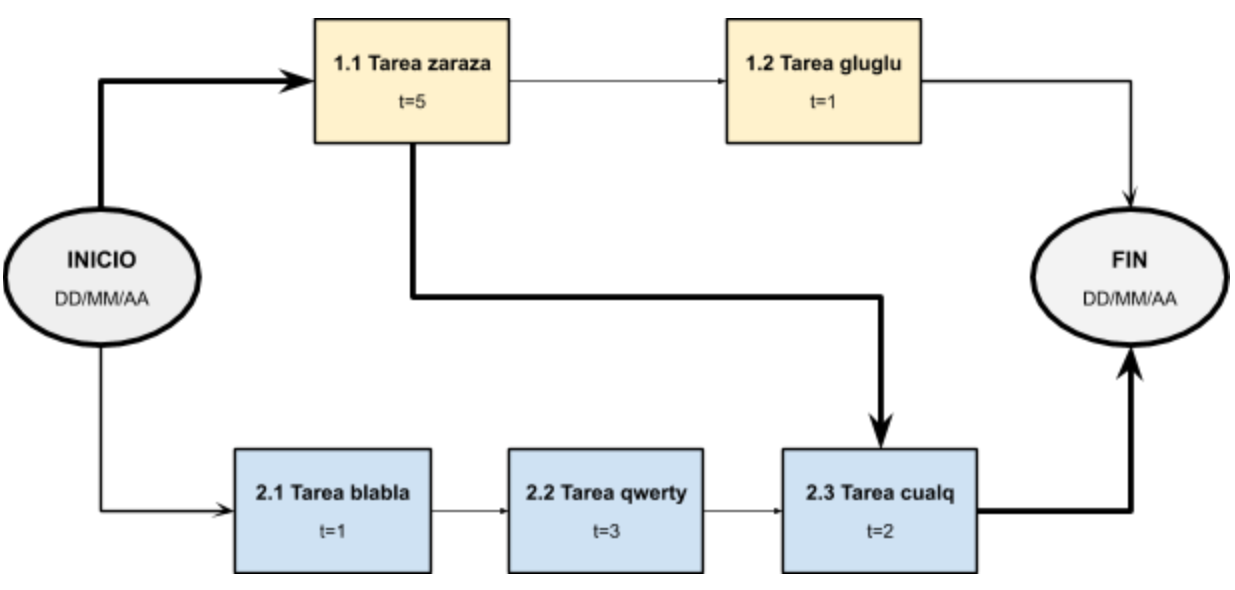
\includegraphics[width=.8\textwidth]{./Figuras/AoN.png}
\caption{Diagrama de \textit{Activity on Node}.}
\label{fig:AoN}
\end{figure}

Indicar claramente en qué unidades están expresados los tiempos.
De ser necesario indicar los caminos semi críticos y analizar sus tiempos mediante un cuadro.
Es recomendable usar colores y un cuadro indicativo describiendo qué representa cada color.

\end{consigna}

\section{11. Diagrama de Gantt}
\label{sec:gantt}

\begin{consigna}{red}
Existen muchos programas y recursos \textit{online} para hacer diagramas de Gantt, entre los cuales destacamos:

\begin{itemize}
\item Planner
\item GanttProject
\item Trello + \textit{plugins}. En el siguiente link hay un tutorial oficial: \\ \url{https://blog.trello.com/es/diagrama-de-gantt-de-un-proyecto}
\item Creately, herramienta online colaborativa. \\\url{https://creately.com/diagram/example/ieb3p3ml/LaTeX}
\item Se puede hacer en latex con el paquete \textit{pgfgantt}\\ \url{http://ctan.dcc.uchile.cl/graphics/pgf/contrib/pgfgantt/pgfgantt.pdf}
\end{itemize}

Pegar acá una captura de pantalla del diagrama de Gantt, cuidando que la letra sea suficientemente grande como para ser legible. 
Si el diagrama queda demasiado ancho, se puede pegar primero la ``tabla'' del Gantt y luego pegar la parte del diagrama de barras del diagrama de Gantt.

Configurar el software para que en la parte de la tabla muestre los códigos del EDT (WBS).\\
Configurar el software para que al lado de cada barra muestre el nombre de cada tarea.\\
Revisar que la fecha de finalización coincida con lo indicado en el Acta Constitutiva.

En la figura \ref{fig:gantt}, se muestra un ejemplo de diagrama de gantt realizado con el paquete de \textit{pgfgantt}. 
En la plantilla pueden ver el código que lo genera y usarlo de base para construir el propio.

Las fechas pueden ser calculadas utilizando alguna de las herramientas antes citadas. Sin embargo, el siguiente ejemplo
fue elaborado utilizando 
\href{https://docs.google.com/spreadsheets/d/1fBz8NhSpc4tkkhz3KjJCbh1nR_ltDkfEcZi4tZXduqs}{esta hoja de cálculo}.

Es importante destacar que el ancho del diagrama estará dado por la longitud del texto utilizado para las tareas 
(Ejemplo: tarea 1, tarea 2, etcétera) y el valor \textit{x unit}. Para mejorar la apariencia del diagrama, es necesario
ajustar este valor y, quizás, acortar los nombres de las tareas.

\begin{figure}[htpb]
  \begin{center}
    \begin{ganttchart}[
      time slot unit=day,
      time slot format=isodate,
      x unit=0.038cm,
      y unit title=0.7cm,
      y unit chart=0.6cm,
      milestone/.append style={xscale=4}
      ]{2021-03-05}{2021-12-16}
      \gantttitlecalendar*{2021-03-05}{2021-12-16}{year} \\
      \gantttitlecalendar*{2021-03-05}{2021-12-16}{month} \\
      \ganttgroup{Duración Total}{2021-03-05}{2021-12-16} \\
      %%%%%%%%%%%%%%%%%Organización
      \ganttgroup{Organización}{2021-03-05}{2021-04-16} \\
      \ganttbar{Planificación del proyecto}{2021-03-05}{2021-04-15} \\
      %%%%%%%%%%%%%%%%%Ejecución
      \ganttgroup{Ejecución}{2021-04-16}{2021-10-21} \\
      \ganttbar{Tarea 1}{2021-04-16}{2021-04-29} \\
      \ganttbar{Tarea 2}{2021-04-30}{2021-05-13} \\
      \ganttbar{Tarea 3}{2021-05-14}{2021-05-27} \\
      \ganttbar{Tarea 4}{2021-05-28}{2021-07-12} \\
      \ganttbar{Tarea 5}{2021-07-13}{2021-08-09} \\
      \ganttbar{Tarea 6}{2021-08-10}{2021-09-23} \\
      \ganttbar{Tarea 7}{2021-09-24}{2021-09-30} \\
      \ganttbar{Tarea 8}{2021-10-01}{2021-10-14} \\
      \ganttbar{Tarea 9}{2021-10-15}{2021-10-21} \\
      % %%%%%%%%%%%%%%%%%Finalización
      \ganttgroup{Finalización}{2021-10-22}{2021-12-16} \\
      \ganttbar{Memoria v1}{2021-10-22}{2021-11-04} \\
      \ganttbar{Memoria v2}{2021-11-05}{2021-11-18} \\
      \ganttbar{Memoria final}{2021-11-19}{2021-12-02} \\
      % La fecha del siguiente milestone es la fecha en que terminamos la memoria
      \ganttmilestone{Enviar memoria al director}{2021-12-02} \\
      \ganttbar{Elaborar la presentación}{2021-12-03}{2021-12-16} \\
      \ganttmilestone{Ensayo de la presentación}{2021-12-16} \\
      %%%%%%%%%%%%%%%%%%%%%%%%%%%%%%%%%%%%%%%%%%%%%%%%%%%%%%%%%%%%%%%
    \end{ganttchart}
  \end{center}
  \caption{Diagrama de gantt de ejemplo}
  \label{fig:gantt}
\end{figure}


\begin{landscape}
\begin{figure}[htpb]
\centering 
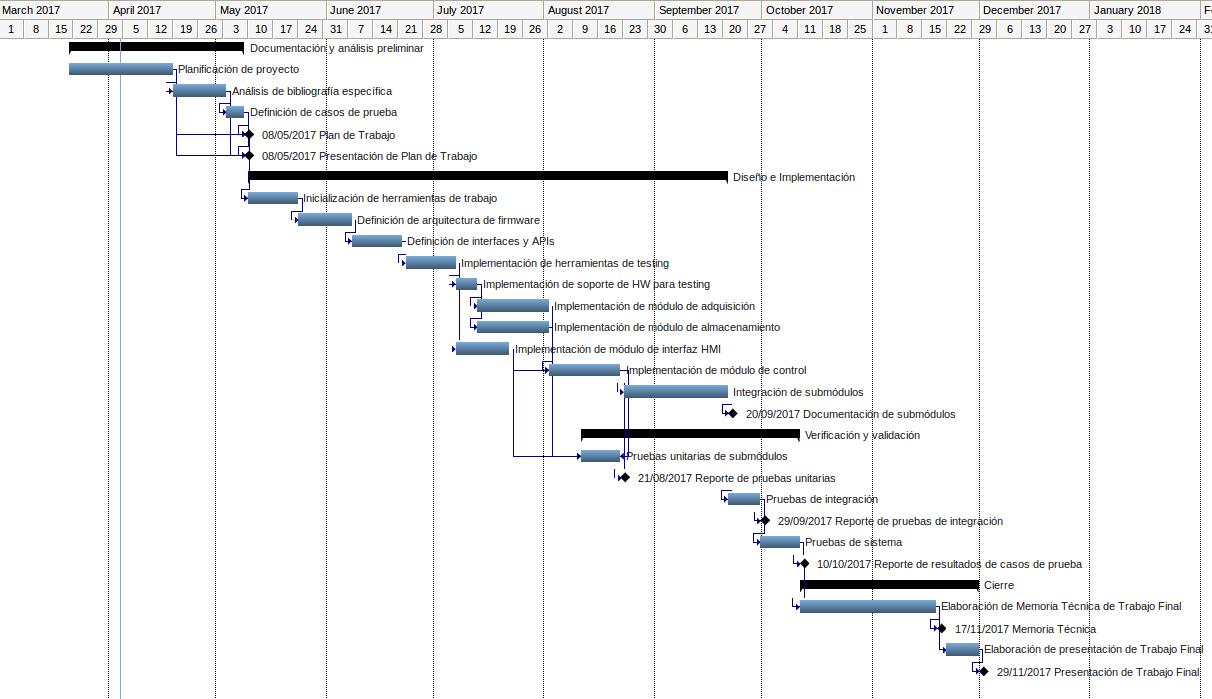
\includegraphics[height=.85\textheight]{./Figuras/Gantt-2.png}
\caption{Ejemplo de diagrama de Gantt (apaisado).} %Modificar este título acorde.
\label{fig:diagGantt}
\end{figure}

\end{landscape}

\end{consigna}


\section{12. Presupuesto detallado del proyecto}
\label{sec:presupuesto}
Los precios expresados en la siguiente tabla se encuentran en Bolivianos Bs.

\begin{table}[htpb]
\centering
\begin{tabularx}{\linewidth}{@{}|X|c|r|r|@{}}
\hline
\rowcolor[HTML]{C0C0C0} 
\multicolumn{4}{|c|}{\cellcolor[HTML]{C0C0C0}COSTOS DIRECTOS} \\ \hline
\rowcolor[HTML]{C0C0C0} 
Descripción &
  \multicolumn{1}{c|}{\cellcolor[HTML]{C0C0C0}Cantidad} &
  \multicolumn{1}{c|}{\cellcolor[HTML]{C0C0C0}Valor unitario} &
  \multicolumn{1}{c|}{\cellcolor[HTML]{C0C0C0}Valor total} \\ \hline
 Tarjeta de desarrollo&
  \multicolumn{1}{c|}{1}&
  \multicolumn{1}{c|}{150} &
  \multicolumn{1}{c|}{150} \\ \hline
Módulo de comunicación GSM/GPRS&
  \multicolumn{1}{c|}{1} &
  \multicolumn{1}{c|}{350} &
  \multicolumn{1}{c|}{350} \\ \hline
Componentes electrónicos para el PCB&
  \multicolumn{1}{c|}{1} &
  \multicolumn{1}{c|}{400} &
  \multicolumn{1}{c|}{400} \\ \hline 
Fabricación y emsamblaje del PCB&
  \multicolumn{1}{c|}{5} &
  \multicolumn{1}{c|}{50} &
  \multicolumn{1}{c|}{250} \\ \hline 
Pantalla nextion&
  \multicolumn{1}{c|}{1} &
  \multicolumn{1}{c|}{260} &
  \multicolumn{1}{c|}{260} \\ \hline 
Caja de la tarjeta PCB&
  \multicolumn{1}{c|}{1} &
  \multicolumn{1}{c|}{250} &
  \multicolumn{1}{c|}{250} \\ \hline
Horas de ingenieria &
  \multicolumn{1}{c|}{680} &
  \multicolumn{1}{c|}{50} &
  \multicolumn{1}{c|}{34000} \\ \hline  

\multicolumn{3}{|c|}{SUBTOTAL}   &
  \multicolumn{1}{c|}{35660} \\ \hline
\rowcolor[HTML]{C0C0C0} 
\multicolumn{4}{|c|}{\cellcolor[HTML]{C0C0C0}COSTOS INDIRECTOS} \\ \hline
\rowcolor[HTML]{C0C0C0} 
Descripción &
  \multicolumn{1}{c|}{\cellcolor[HTML]{C0C0C0}Cantidad} &
  \multicolumn{1}{c|}{\cellcolor[HTML]{C0C0C0}Valor unitario} &
  \multicolumn{1}{c|}{\cellcolor[HTML]{C0C0C0}Valor total} \\ \hline
\multicolumn{1}{|l|}{30 \% de los costos directos} &
   1&
   1&10698
   \\ \hline
\multicolumn{3}{|c|}{SUBTOTAL} &
  \multicolumn{1}{|c|}{10698} \\ \hline
\rowcolor[HTML]{C0C0C0}
\multicolumn{3}{|c|}{TOTAL} &46358
   \\ \hline
\end{tabularx}%
\end{table}


\section{13. Gestión de riesgos}
\label{sec:riesgos}
a) Identificación de los riesgos y estimación de sus consecuencias:

Riesgo 1: Detección de errores en el esquemático o el ruteo del PCB ya habiendo fabricado los prototipos.
\begin{itemize}
	\item Severidad (7): Se retrasa el proyecto por unas semanas hasta volver a mandar a fabricar los PCBs nuevamente.
	\item Probabilidad de ocurrencia (6): Dada la moderada experiencia del alumno es posible que ocurra.
\end{itemize}  

Riesgo 2: Mala estimación de la planificación.
\begin{itemize}
	\item Severidad (8): El proyecto sufrirá varios cambios y retrasos en la ejecución.
	\item Probabilidad de ocurrencia (6): No cuenta con mucha experiencia en planificación de proyectos IoT.
\end{itemize}

Riesgo 3: Retraso en la programación del firmware.
\begin{itemize}
	\item Severidad (7): Retrasos en el proyecto debido a que el firmware es una parte fundamental en el momento de la integración e implementación del prototipo.
	\item Probabilidad de ocurrencia (5): Falta de conocimiento de la arquitectura del microcontrolador.
\end{itemize}  

Riesgo 4: Retraso en la fabricación y ensamblaje de los PCBs.
\begin{itemize}
	\item Severidad (7): Por falta del hardware no se podrá probar el firmware sobre el hardware del prototipo.
	\item Probabilidad de ocurrencia (4): Se mandará a fabricar y ensamblar a una empresa china. 
\end{itemize}

Riesgo 5: Pérdida o daño de los archivos asociados al proyecto.
\begin{itemize}
	\item Severidad (7): Al perder los archivos del proyecto se tendrá que volver reiniciar diseños.
	\item Probabilidad de ocurrencia (3): Se llevará un control de versiones con los documentos del proyecto.
\end{itemize}  

b) Tabla de gestión de riesgos: 

\begin{table}[htpb]
\centering
\begin{tabularx}{\linewidth}{@{}|X|c|c|c|c|c|c|@{}}
\hline
\rowcolor[HTML]{C0C0C0} 
Riesgo & S & O & RPN & S* & O* & RPN* \\ \hline
Detección de errores en el esquemático o el ruteo del PCB ya habiendo fabricado los prototipos&   7&   6&     42&    7&    5&      35\\ \hline
Mala estimación de la planificación      &   8&   6&     48&    8&    4&      32\\ \hline
Retraso en la programación del firmware       &   7&   5&     35&    &    &      \\ \hline
Retraso en la fabricación y ensamblaje de los PCBs       &   7&   4&     28&    &    &      \\ \hline
Pérdida o daño de los archivos asociados al proyecto      &   7&   3&     21&    &    &      \\ \hline
\end{tabularx}%
\end{table}

Criterio adoptado: 

Se tomarán medidas de mitigación en los riesgos cuyos números de RPN sean mayores a 42

Nota: los valores marcados con (*) en la tabla corresponden luego de haber aplicado la mitigación.

c) Plan de mitigación de los riesgos que originalmente excedían el RPN máximo establecido:
 
Riesgo 1*:  Se revisará minuciosamente los esquemáticos, el ruteo del PCB, y se buscará ayuda en algún ingeniero que tenga experiencia en desarrollo de circuitos impresos en proyectos de estas características.
  \begin{itemize}
	\item Severidad (7):No cambia.
	\item Probabilidad de ocurrencia (5): Será menor al contar con ayuda de profesionales expertos en el tema.
\end{itemize}

Riesgo 2*: Se consultará con el director en el momento de realizar la planificación para ajustar los tiempos de las tareas de acuerdo a su experiencia en este tipo de proyectos.
  \begin{itemize}
	\item Severidad (8):No cambia.
	\item Probabilidad de ocurrencia (4): Se reduce el riesgo de hacer una mala planificación.
\end{itemize}


\section{14. Gestión de la calidad}
\label{sec:calidad}
Para cada uno de los requerimiento funcionales, a constitución, se lista su respectiva validacion y verificación. Las mismas llevadas a cabo por el responsable del proeyecto.

\begin{itemize} 
	\item Req \#1: El firmware debe estar bajo un RTOS.
	\begin{itemize}
		\item Verificación: Envio de datos por colas entre tareas.
		\item Validación: Mostrar el intercambio de datos entre tareas por monitor serial. 
	\end{itemize}

	\item Req \#2: Se deberá llevar control de los cambios bajo el sistema de control de versiones Git.
	\begin{itemize}
		\item Verificación: Utilizar una consola de comandos para mandar comandos git en los archivos del proyecto.
		\item Validación: Mostrar los todos commits realizados durante el proyecto.  
	\end{itemize}

	\item Req \#3: El firmware debe poder suscribirse y publicar en tópicos de un broker MQTT.
	\begin{itemize}
		\item Verificación: Publicar datos a un tópico del broker MQTT.
		\item Validación: Visualizar los datos en la interfaz gráfica en la plataforma IoT. 
	\end{itemize}

	\item Req \#4: El firmware debe comunicarse con el módulo GSM/GPRS mediante protocolo serial.
	\begin{itemize}
		\item Verificación: Mandar comandos AT por puerto serial y esperar la respuesta del modulo.
		\item Validación: Visualizar las respuesta del  módulo en un monitor serial.  
	\end{itemize}

	\item Req \#5: Se deben realizar los drivers para los sensores.
	\begin{itemize}
		\item Verificación: Hacer un test unitario para cada driver.
		\item Validación: Mostrar los resultados de cobertura en GCOV. 
	\end{itemize}

	\item Req \#6: El PCB tiene que tener un circuito de acondicionamiento para una entrada RS485.
	\begin{itemize}
		\item Verificación: Hacer la lectura del sensor conectado por RS485.
		\item Validación: Inspección por parte de cliente del circuito en el PCB.  
	\end{itemize}

	\item Req \#7: Debe contar con una display.
	\begin{itemize}
		\item Verificación: Mandar datos al display para visualizarlos.
		\item Validación: Mostrar lecturas de los sensores en gráficas en el display.  
	\end{itemize}

	\item Req \#8: Debe mostrar los valores de los sensores.
	\begin{itemize}
		\item Verificación: Mandar datos leídos de los sensores a un tópico por MQTT a la plataforma.
		\item Validación: Entrar a la plataforma IoT y visualizar los datos. 
	\end{itemize}

	\item Req \#9: Debe contar con botones para controlar la actuadores.
	\begin{itemize}
		\item Verificación: Visualizar los datos recibidos en un monitor serial al momento de presionar un botón en la plataforma IoT.
		\item Validación: Oprimir un botón en la interfaz y visualizar la activación de un actuador. 

	\item Req \#10: Requerimientos de documentación.
	\begin{itemize}
		\item Verificación: Verificar que se haya presentado el informe de avance y la memoria técnica del proyecto.
		\item Validación: Revisar que se cumplio los requerimientos estipulados en el plan de proyectos. 
	\end{itemize}
\end{itemize}
\end{itemize}

\section{15. Procesos de cierre}    
\label{sec:cierre}

\begin{itemize}
	\item Pautas de trabajo que se seguirán para analizar si se respetó el Plan de Proyecto original:
	\begin{itemize}
		\item Encargado: Ing. Mario Aguilar Montoya
		\item Procedimiento: Durante el proceso de cierre se evaluara si se han cumplido los plazos
		de entrega y ejecucion de cada tarea planteada en el Plan de Proyecto. En el caso de hallar requerimientos incumplidos y/o retrasos en las
		tareas se evaluaran las causa y se propondran acciones para evitarlo en futuros
		proyectos.
	\end{itemize}
	\item Identificación de las técnicas y procedimientos útiles e inútiles que se emplearon, los problemas que surgieron y cómo se solucionaron:
	\begin{itemize}
		\item Encargado: Ing. Mario Aguilar Montoya
		\item Procedimiento: Se evaluaran los procedimientos utilizados en funcion a su utilidad
		y eficiencia para alcanzar los objetivos predefinidos.
	\end{itemize}
	\item Acto de cierre:
	\begin{itemize}
		\item Encargado: Ing. Mario Aguilar Montoya
		\item Procedimiento: Se realizara la defensa publica del trabajo final ante el jurado, posterior a esto se
		procedera a agradecer a todos los que ayudaron a realizar el proyecto, director del
		trabajo, miembros del jurado y autoridades de la CESE.
	\end{itemize}
\end{itemize}

\end{document}